\section{Results}
\label{sec:results}


- Figure results.1: Overall error at the end of the trial with unlimited sampling and without weighing by the rarity (1/prob of occurrence) of the class
- Figure results.2: overall error at the end of the trial with unlimited sampling and with weighing by the rarity of the class
- Figure results.3: Overall performance when combining limited time and limited sample budgets.

% Different arrival rates and different distributions.

\begin{figure}[htpd]
	\centering
	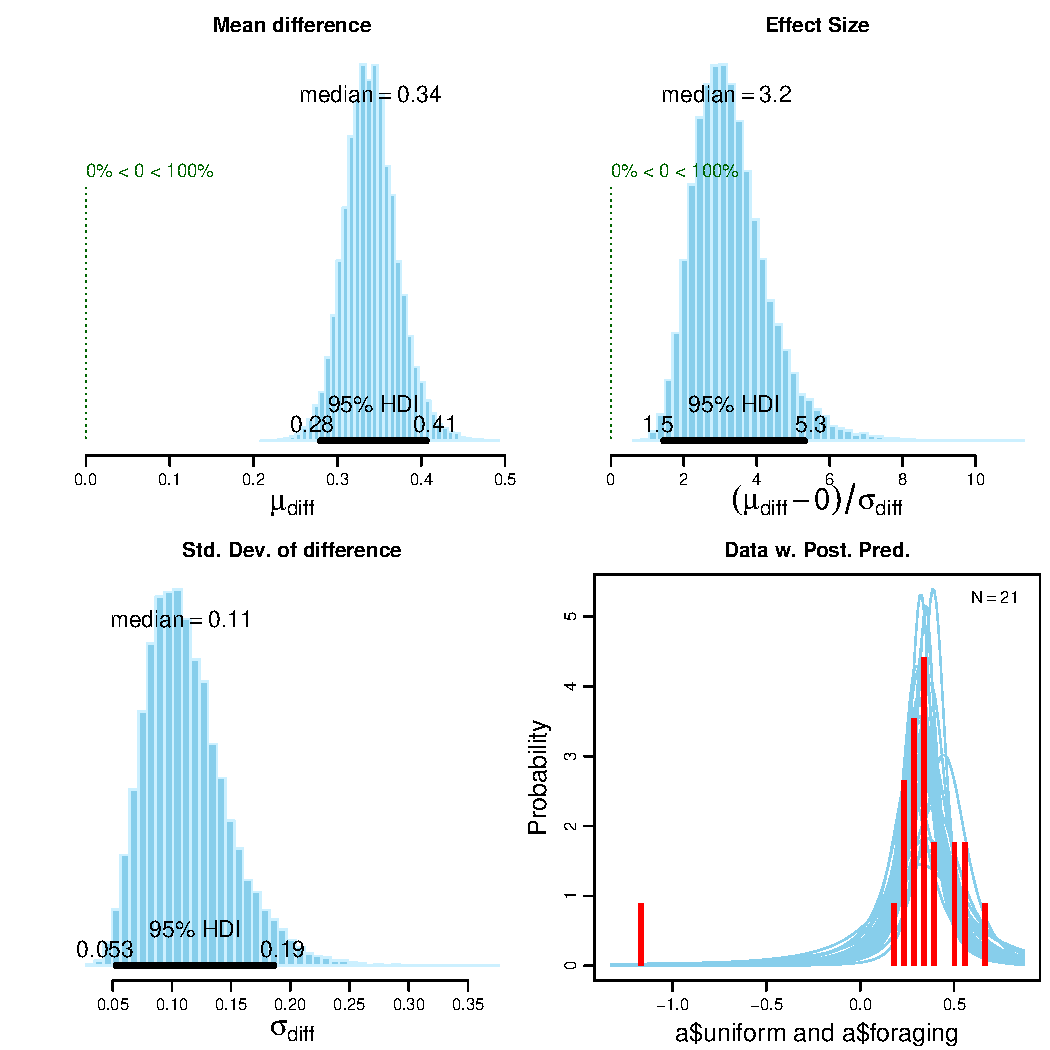
\includegraphics[width=0.8\textwidth]{images/diff-diff.pdf}
	\caption{Analysis of the basic scenario with different arrival rates and standard deviations.  We see here the effect size in the reduction in terminal error is 3.2, by Cohen's d measure.  This qualifies as a ``very large'' effect.}
	\label{fig:diff-diff}
\end{figure}
